
\chapter{Descrição do Projeto}
\label{chap:descricao-projeto}


O dispositivo propõe metodologia inovadora para derriça de grãos, substituindo as hastes vibratórias utilizadas atualmente, por sistema sonoro que promoverá a vibração dos grãos até o desprendimento do mesmo. Esta metodologia permite a derriça seletiva devido à especificidade e controle da frequência de vibração transmitida ao fruto. Será desenvolvido metodologia para aquisição de parâmetro de dispersão sonora e simulações para definir a melhor disposição dos autofalantes. Posteriormente será desenvolvido protótipo à ser validado no campo e análises da frequencia ideal a ser utilizada para derriça seletiva de grãos.

\chapter{Objetivo da Pesquisa}
\label{chap:objetivo-pesquisa}

Identificar se há patentes ou artigos de dispositivos idênticos ou semelhantes no processo de derriça acústica do café.

\chapter{Base de Dados}
\label{chap:base-dados}

\begin{BaseDados}
  \itemBaseDados{INPI}{busca em patentes depositadas no Brasil.}
  \itemBaseDados{ESPACENET}{busca internacional no escritório Europeu de patentes.}
  \itemBaseDados{WEB OF SCIENCE}{busca internacional de artigos.}
\end{BaseDados}

\chapter{Códigos de classificação (IPI)}
\label{chap:codigos-classificacao}

\begin{CodigoClassIPC}
  \itemCodigoClassIPC{A01D 46/00}{Colheita de frutas, legumes, lúpulos ou similares; Dispositivos para sacudir árvores ou arbustos.}%
  \itemCodigoClassIPC{A01D 46/06}{de café.}
  \itemCodigoClassIPC{A01D 46/26}{Dispositivos para sacudir árvores ou arbustos; Dispositivos para coleta de frutos utilizável com os mesmos.} 
\end{CodigoClassIPC}

\chapter{Palavras Chave}
\label{chap:palavras-chave}

\begin{PalavrasChave}
  \itemPalavrasChave{Português}{Café; Derriça; Acústica; Seletiva}
  \itemPalavrasChave{Inglês}{Coffee; Harvesting; Acoustic; Selective}
\end{PalavrasChave}



\chapter{Metodologia}
\label{chap:metodologia}

Iniciou-se a pesquisa definindo-se quais seriam as bases de dados de patentes para a efetuação da pesquisa. As bases escolhidas são justificadas por serem instituições regulamentadas e reconhecidas por vários países; sendo uma de abrangência nacional --- \emph{INPI} --- e outra internacional --- \emph{ESPACENET}. Para a pesquisa de artigos utilizou-se da base de dados \emph{WEB OF SCIENCE}, por a mesma ser reconhecida internacionalmente por órgãos e instituições de ensino sendo o único lugar onde se pode obter mais de um bilhão de referências citadas pesquisáveis \cite{web-of-science-2016}.

\begin{figure}[!htp]
  \centering
  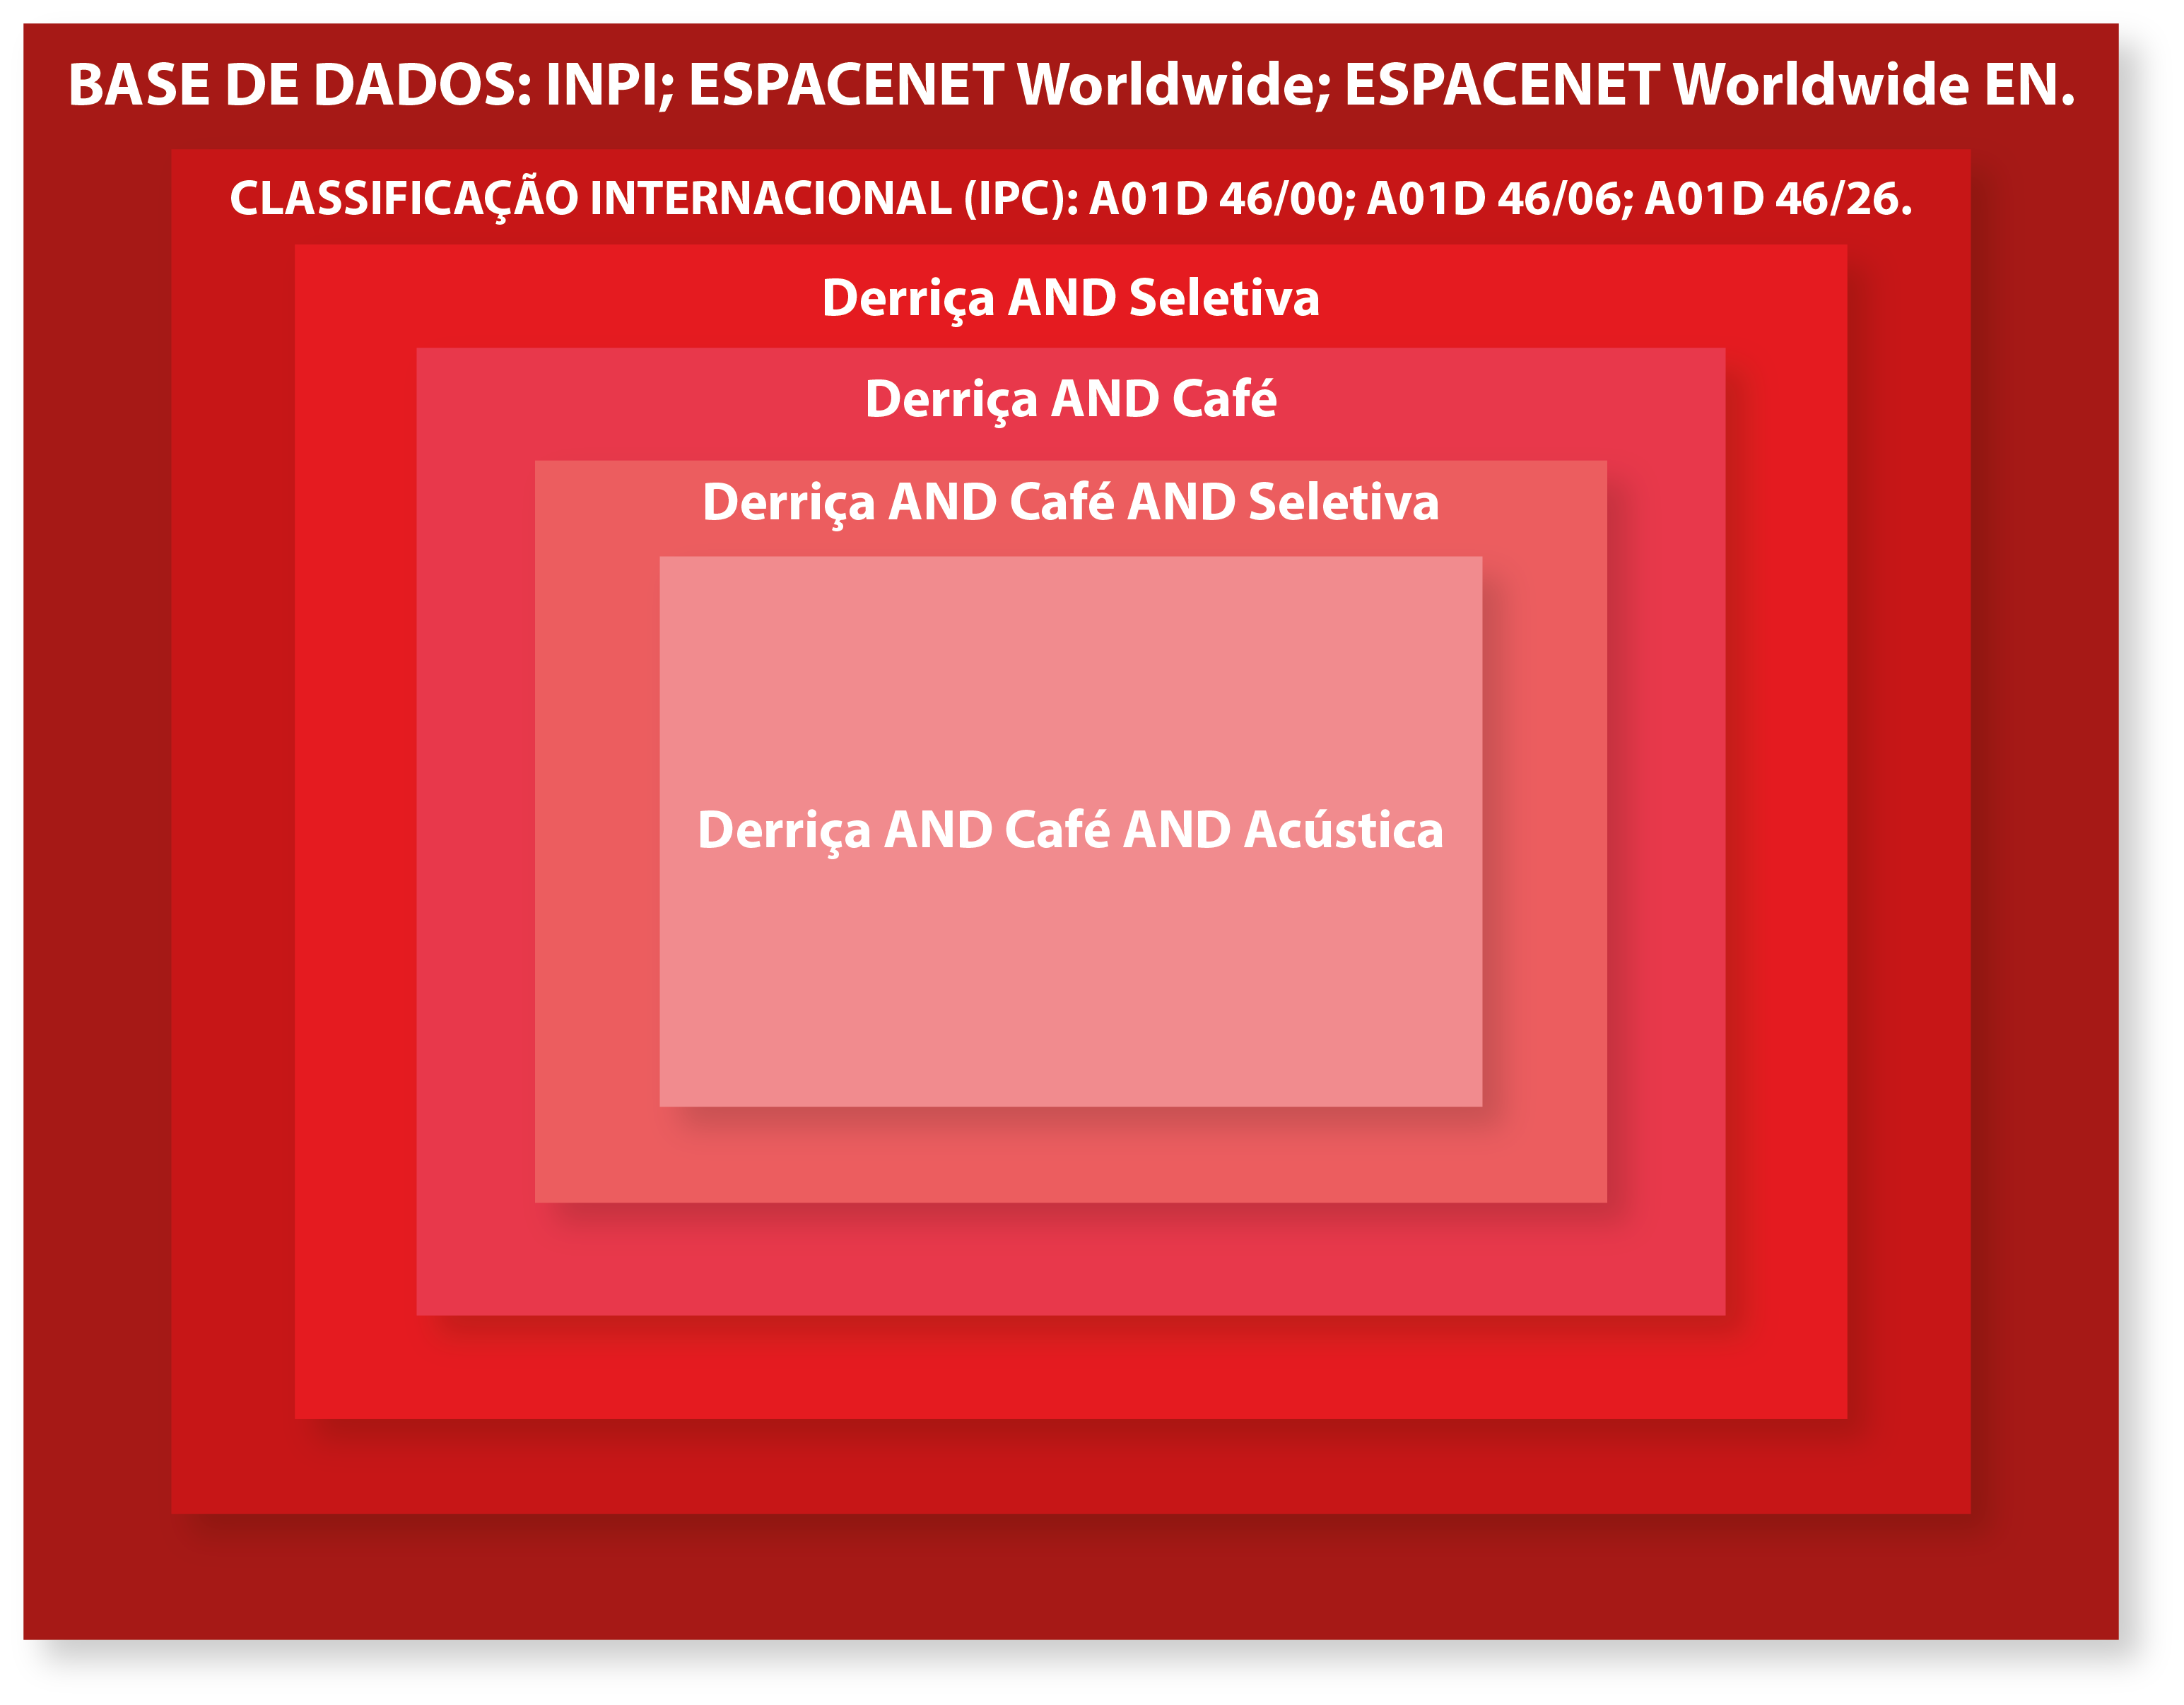
\includegraphics[width=.9\textwidth]{fig-01}
  \caption{Ordem dos escopos da pesquisa.}
  \label{fig:escopo-pesquisa}
\end{figure}

Em um segundo instante, selecionou-se os três códigos de classificação IPC de maior relevância ao tema pesquisado. Então definiu-se as palavras chaves e fez-se combinações com as mesmas em uma ordem que fosse de um ponto mais genérico ao específico. A Figura~\ref{fig:escopo-pesquisa} ilustra a ordem objetiva da metodologia.

As combinações entre os códigos IPC e palavras chaves estão descritas nas Tabelas~\ref{tab:palavras-chave-inpi},~\ref{tab:palavras-chave-espacenet},~e~\ref{tab:palavras-chave-espacenet-en} e na Tabela~\ref{tab:resultado-web-science} as expressões utilizadas na base de dados \emph{WEB OF SCIENCE}.

\begin{table}[!htp]
  \centering
  \caption{Combinações entre IPC e palavras chaves para cada pesquisa na base de dados do \emph{INPI}.}
  \label{tab:palavras-chave-inpi}
  \begin{tabular}{m{4.5em} m{3em}  c c c c c c}
    \hline
    \multicolumn{8}{c}{\large\textbf{Patentes}}\\
    \hline
    \textbf{Base de dados} & \textbf{IPC} & \textbf{Palavra 1} & \textbf{Op.} & \textbf{Palavra 2} & \textbf{Op.} & \textbf{Palavra 3} & \textbf{Resultado} \\
    \hline
    \multirow{12}{.1\linewidth}{INPI} & \multirow{4}{.1\linewidth}{AD01 46/00} & Derriça & AND & Seletiva & - & - & 0 \\
                           & & Derriça & AND & Café & - & - & 0 \\
                           & & Derriça & AND & Café & AND & Seletiva & 0 \\
                           & & Derriça & AND & Café & AND & Acústica & 0 \\
    \cline{2-8}
                           & \multirow{4}{.1\linewidth}{A01D 46/06} & Derriça & AND & Seletiva & - & - & 0 \\
                           & & Derriça & AND & Café & - & - & 11 \\
                           & & Derriça & AND & Café & AND & Seletiva & 0 \\
                           & & Derriça & AND & Café & AND & Acústica & 0 \\
    \cline{2-8}
                           & \multirow{4}{.1\linewidth}{A01D 46/26} & Derriça & AND & Seletiva & - & - & 0 \\
                           & & Derriça & AND & Café & - & - & 0 \\
                           & & Derriça & AND & Café & AND & Seletiva & 0 \\
                           & & Derriça & AND & Café & AND & Acústica & 0 \\
    \hline
  \end{tabular}
\end{table}

\begin{table}[!htp]
  \centering
  \caption{Combinações entre IPC e palavras chaves para cada pesquisa na base de dados do \emph{ESPACE NET Worldwide}.}
  \label{tab:palavras-chave-espacenet}
  \begin{tabular}{m{4.5em} m{3em}  c c c c c c}
    \hline
    \multicolumn{8}{c}{\large\textbf{Patentes}}\\
    \hline
    \textbf{Base de dados} & \textbf{IPC} & \textbf{Palavra 1} & \textbf{Op.} & \textbf{Palavra 2} & \textbf{Op.} & \textbf{Palavra 3} & \textbf{Resultado} \\
    \hline
    \multirow{12}{.1\linewidth}{ESPACE NET Worldwide} & \multirow{4}{.1\linewidth}{A01D 46/00} & Harvesting & AND & Selective & - & - & 12 \\
                           & & Harvesting & AND & Coffee & - & - & 4 \\
                           & & Harvesting & AND & Coffee & AND & Selective & 0 \\
                           & & Harvesting & AND & Coffee & AND & Acoustic & 0 \\
    \cline{2-8}
                           & \multirow{4}{.1\linewidth}{A01D 46/06} & Harvesting & AND & Selective & - & - & 1 \\
                           & & Harvesting & AND & Coffee & - & - & 9 \\
                           & & Harvesting & AND & Coffee & AND & Selective & 1 \\
                           & & Harvesting & AND & Coffee & AND & Acoustic & 0 \\
    \cline{2-8}
                           & \multirow{4}{.1\linewidth}{A01D 46/26} & Harvesting & AND & Selective & - & - & 2 \\
                           & & Harvesting & AND & Coffee & - & - & 5 \\
                           & & Harvesting & AND & Coffee & AND & Selective & 0 \\
                           & & Harvesting & AND & Coffee & AND & Acoustic & 0 \\
    \hline
  \end{tabular}
\end{table}


\begin{table}[!htp]
  \centering
  \caption{Combinações entre IPC e palavras chaves para cada pesquisa na base de dados do \emph{ESPACE NET Worldwide EN}.}
  \label{tab:palavras-chave-espacenet-en}
  \begin{tabular}{m{4.5em} m{3em}  c c c c c c}
    \hline
    \multicolumn{8}{c}{\large\textbf{Patentes}}\\
    \hline
    \textbf{Base de dados} & \textbf{IPC} & \textbf{Palavra 1} & \textbf{Op.} & \textbf{Palavra 2} & \textbf{Op.} & \textbf{Palavra 3} & \textbf{Resultado} \\
    \hline
    \multirow{12}{.1\linewidth}{ESPACE NET Worldwide EN} & \multirow{4}{.1\linewidth}{A01D 46/00} & Harvesting & AND & Selective & - & - & 78 \\
                           & & Harvesting & AND & Coffee & - & - & 39 \\
                           & & Harvesting & AND & Coffee & AND & Selective & 3 \\
                           & & Harvesting & AND & Coffee & AND & Acoustic & 0 \\
    \cline{2-8}
                           & \multirow{4}{.1\linewidth}{A01D 46/06} & Harvesting & AND & Selective & - & - & 2 \\
                           & & Harvesting & AND & Coffee & - & - & 13 \\
                           & & Harvesting & AND & Coffee & AND & Selective & 2 \\
                           & & Harvesting & AND & Coffee & AND & Acoustic & 0 \\
    \cline{2-8}
                           & \multirow{4}{.1\linewidth}{A01D 46/26} & Harvesting & AND & Selective & - & - & 18 \\
                           & & Harvesting & AND & Coffee & - & - & 47 \\
                           & & Harvesting & AND & Coffee & AND & Selective & 3 \\
                           & & Harvesting & AND & Coffee & AND & Acoustic & 0 \\
    \hline
  \end{tabular}
\end{table}


\begin{table}[!htp]
  \centering
  
  \caption{Expressões para pesquisa na base de dados \emph{WEB OF SCIENCE}.}
  \label{tab:resultado-web-science}
  \begin{tabular}{c c c}
    \hline
    \multicolumn{3}{c}{\large\textbf{Artigos}} \\
    \hline
    \textbf{Base de dados} & \textbf{Expressão} & \textbf{Resultado} \\
    \hline
    \multirow{4}{.2\linewidth}{Web of science} & coffee selective harvesting & 7 \\
    \cline{2-3}
                           & coffee harvesting machine & 12 \\
    \cline{2-3}
                           & coffee acoustic harvesting machine & 0 \\
    \cline{2-3}
                           & coffee harvesting acoustic & 2 \\
    \hline
  \end{tabular}
\end{table}



\chapter{Resultado das pesquisas}
\label{chap:resultado-pesquisa}

Os resultados das buscas estão descritos nos anexos conforme a ordem abaixo:

\begin{Resultados}
  \itemResultado{INPI}{Anexo~\ref{chap:inpi}}
  \itemResultado{ESPACENET Worldwide}{Anexo~\ref{chap:espacenet}}
  \itemResultado{ESPACE NET Worldwide EN}{Anexo~\ref{chap:espacenet-en}}
  \itemResultado{WEB OF SCIENCE}{Anexo~\ref{chap:web-science}}
\end{Resultados}


\chapter{Parecer técnico do resultado da pesquisa}
\label{chap:parecer-tecnico}

Nos resultados da metodologia adotada, aferiu-se que não há nenhum dispositivo semelhante ou idêntico registrado em patente ou citado em artigo. É sugerível que uma nova categoria ou subcategoria de classificação internacional (IPC) seja criada dentro do escopo de A01D46/00, pois o dispositivo não se enquadra em nenhuma categoria existente para a derriça de frutos.

\AssinaturasResultado


%%% Local Variables:
%%% mode: latex
%%% TeX-master: "../template-01"
%%% End:
